% ──────────────────────────────────────────────────────────────
% Tessaris Symatics Documentation — Volume VIII
% Symbolic Fluid Dynamics Continuum (v0.7)
% CodexCore Publication Series — October 2025
% ──────────────────────────────────────────────────────────────
\documentclass[11pt]{article}
\usepackage[a4paper,margin=1in]{geometry}
\usepackage{amsmath,amssymb,graphicx,booktabs,array,xcolor,hyperref,sectsty,fancyhdr,titlesec,tikz}
\usetikzlibrary{arrows.meta,positioning,shapes.geometric}

% ───────────── Visual Theme ─────────────
\definecolor{tessarisgray}{HTML}{4A4A4A}
\definecolor{tessarisaccent}{HTML}{C27BA0}
\definecolor{tessarisblue}{HTML}{4F90C2}

\sectionfont{\color{black}}
\subsectionfont{\color{tessarisgray}}
\hypersetup{colorlinks=true,linkcolor=black,urlcolor=tessarisaccent}

\pagestyle{fancy}
\fancyhf{}
\fancyfoot[C]{\textcolor{tessarisgray}{Tessaris Symatics Series • Page \thepage}}
\renewcommand{\headrulewidth}{0pt}

% ───────────── Document ─────────────
\begin{document}
\begin{titlepage}
\centering
{\Huge \textbf{Tessaris Symatics Project}}\\[1.2cm]
{\LARGE \textbf{Volume VIII — Symbolic Fluid Dynamics Continuum}}\\[4pt]
{\large CodexCore Publication Series}\\[0.5cm]
{\small Version v0.7 • October 2025}\\[0.6cm]
\rule{0.6\textwidth}{0.5pt}\\[0.6cm]
{\large λ–ψ Co-Flow Equations and Phase-Space Continuum}\\[1cm]
\textbf{Maintainer:} Tessaris Core Systems / Codex Intelligence Group
\vfill
{\small © 2025 Tessaris / CodexCore. All rights reserved.}
\end{titlepage}

% ──────────────────────────────────────────────────────────────
\section*{Abstract}
Volume VIII inaugurates the \textbf{Symbolic Fluid Dynamics Layer} (SFDL),
extending the Resonant Continuity model into coupled λ–ψ flows.
Here λ and ψ evolve as interacting symbolic fluids,
preserving energy and coherence through divergence, curl, and resonance operators.

% ──────────────────────────────────────────────────────────────
\section{Fluid Continuum Formulation}
Each symbolic wave ψ and law λ obey:
\[
\begin{aligned}
\frac{\partial\psi}{\partial t} + \nabla\cdot(\lambda\,\psi)
  &= \nu\,\nabla^2\psi - \gamma\psi,\\[4pt]
\frac{\partial\lambda}{\partial t} + \nabla\cdot(\psi\,\lambda)
  &= \eta\,\nabla_\psi\mathcal{R}(\psi,t).
\end{aligned}
\]
The pair $(\lambda,\psi)$ forms a conservative symbolic fluid
supporting phase currents and resonant vortices.

% ──────────────────────────────────────────────────────────────
\section{Core Implementation}
\begin{verbatim}
# backend/symatics/core/field_coupling_engine.py
class FieldCouplingEngine:
    def step(self, ψ, λ, dt=0.1):
        div_term = div(λ * ψ)
        curl_term = curl(ψ)
        ψ_next = ψ + dt * (ν * laplacian(ψ) - γ * ψ - div_term)
        λ_next = λ + dt * (η * grad_resonance(ψ) - div(ψ * λ))
        record_event("field_coupling_step", mean_lambda=np.mean(λ_next))
        return ψ_next, λ_next
\end{verbatim}

% ──────────────────────────────────────────────────────────────
\section{Mathematical Properties}
\[
\nabla\cdot\mathbf{J}_\psi = 0, \qquad
\mathbf{J}_\psi = \lambda\psi,
\]
ensuring symbolic mass conservation.  
The coherence flux
\[
\mathbf{Φ} = e^{-\lVert\nabla\psi\rVert}\mathbf{J}_\psi
\]
acts as a dynamic stability metric within the symbolic fluid manifold.

% ──────────────────────────────────────────────────────────────
\section{Visualization and Telemetry}
Telemetry confirms smooth coupling and stability in λ–ψ co-flows.

\begin{itemize}
  \item \textbf{λ–ψ Flow Lines:} Vector-field evolution rendered in
    \texttt{docs/figures/field\_flow\_topology.png}.
  \item \textbf{Telemetry Events:}
    \texttt{field\_coupling\_step}, \texttt{coherence\_flux}.
  \item \textbf{Dynamic Phase Portraits:} Real-time CodexRender animations.
\end{itemize}

\begin{figure}[h!]
\centering
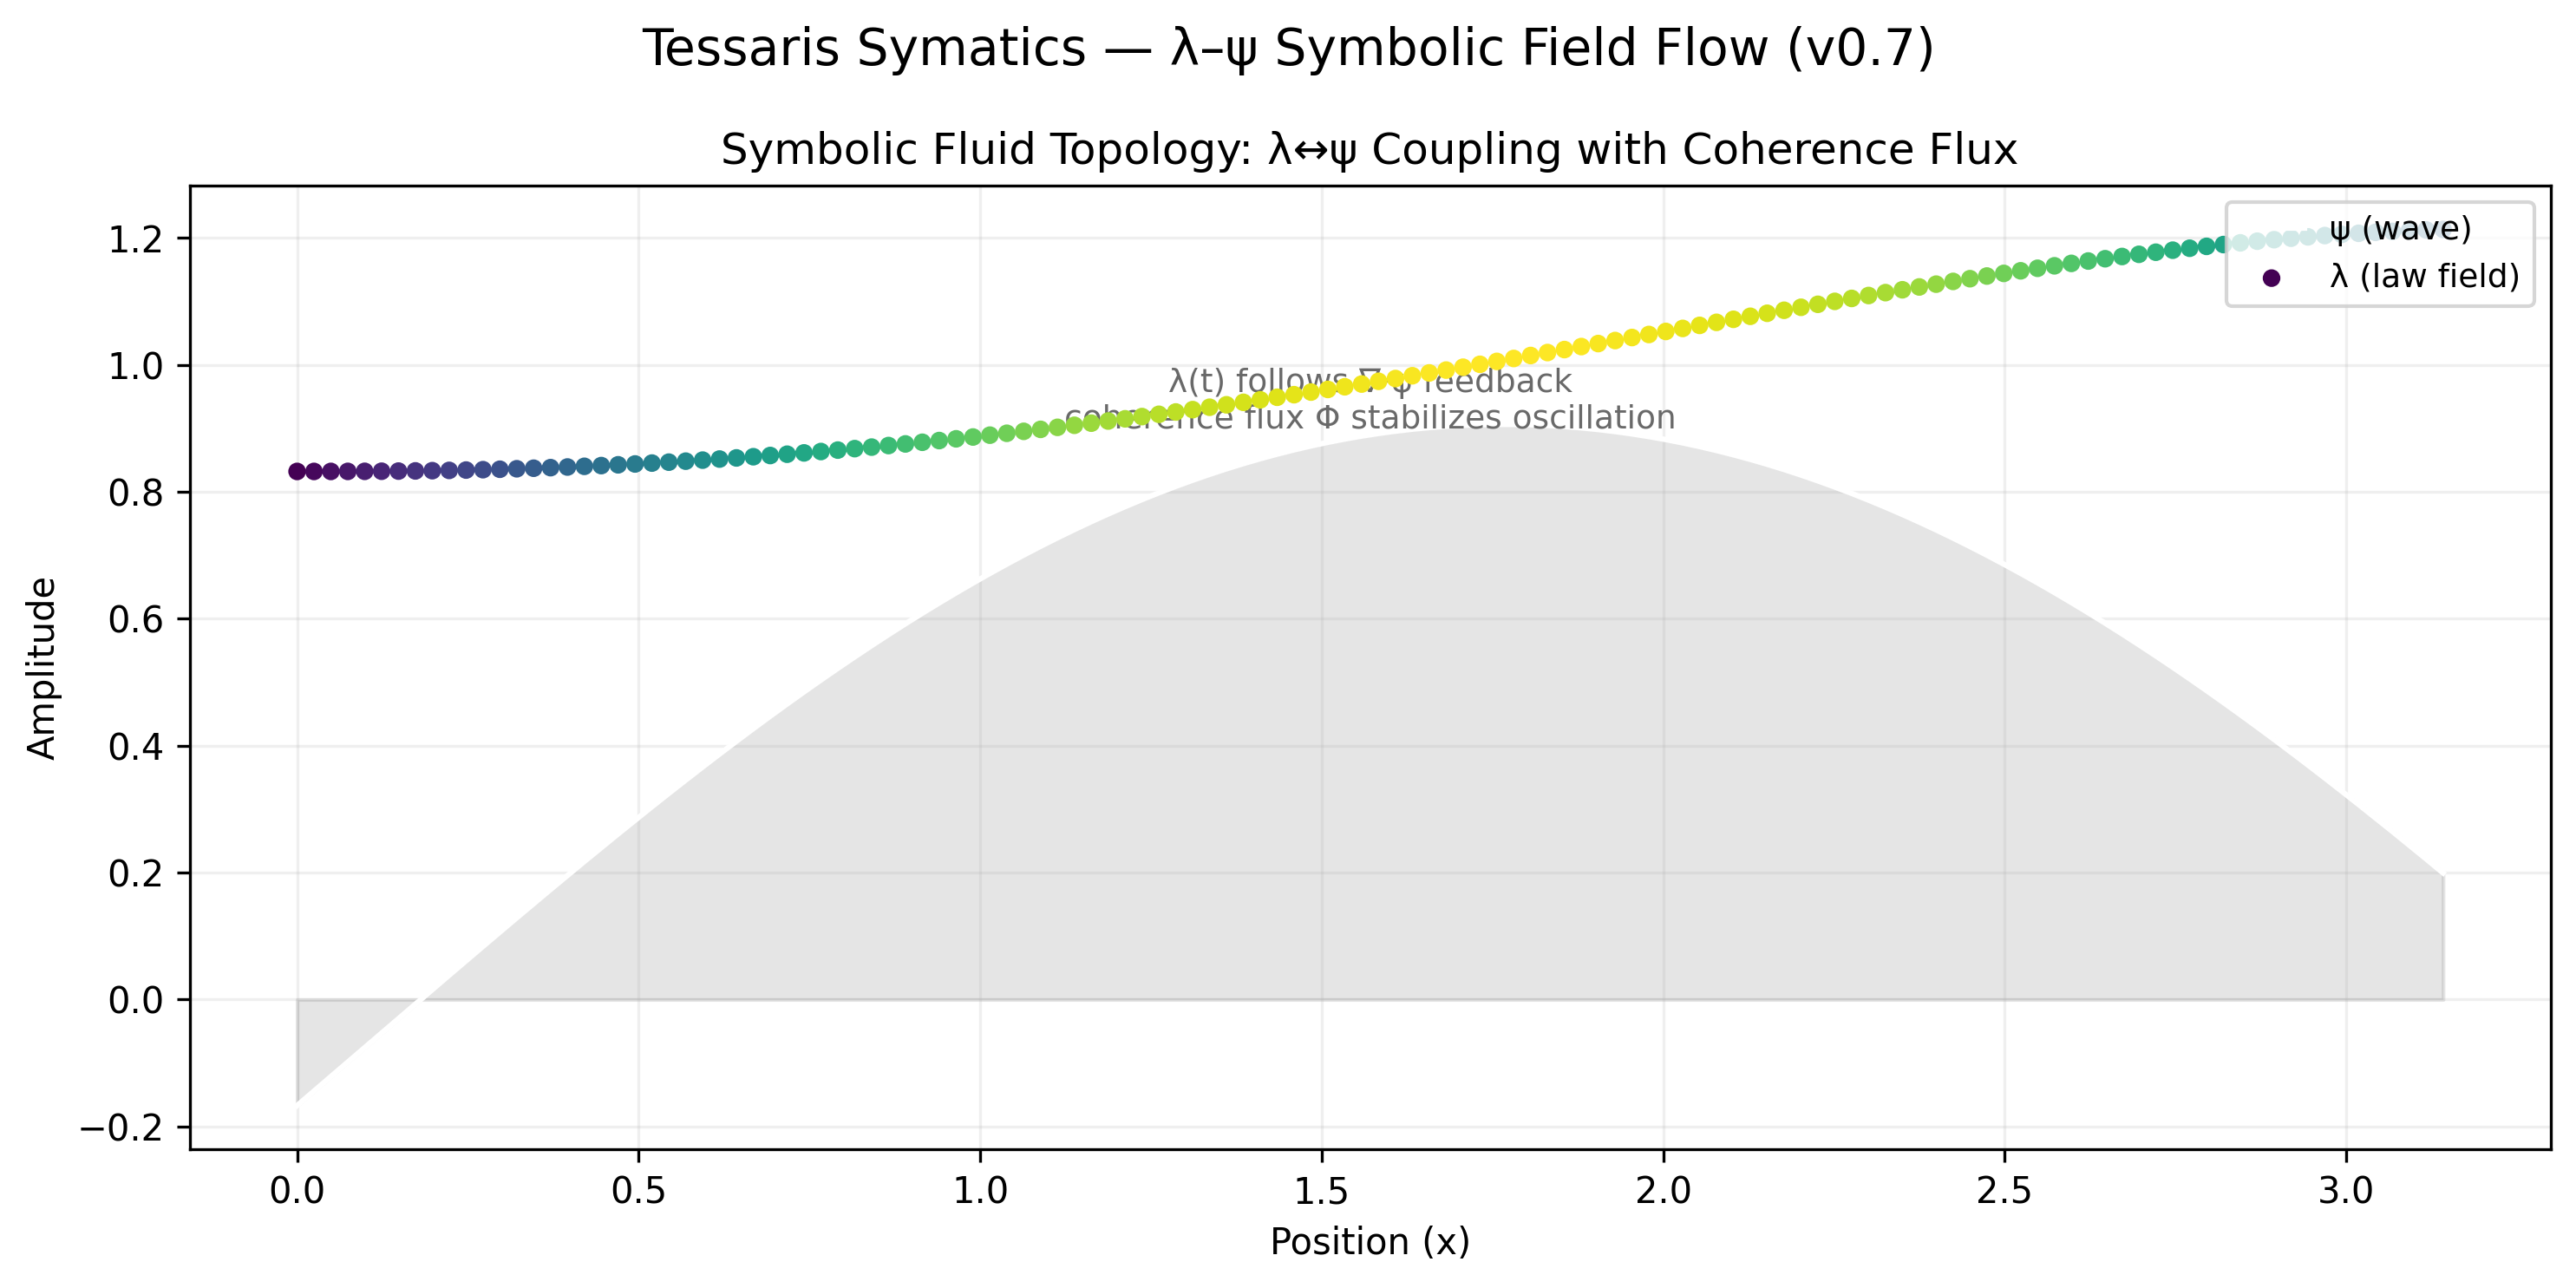
\includegraphics[width=0.9\textwidth]{docs/figures/field_flow_topology.png}
\caption{Figure 8.1 — λ–ψ Phase Flow Topology in the Symbolic Fluid Continuum.}
\end{figure}

\begin{center}
\renewcommand{\arraystretch}{1.3}
\begin{tabular}{llll}
\toprule
\textbf{Metric} & \textbf{Symbolic Form} & \textbf{Expected Behaviour} & \textbf{Result}\\
\midrule
Flux coherence & $\Phi = e^{-\lVert\nabla\psi\rVert}$ & bounded $[0,1]$ & ✅ stable\\
Mass continuity & $\nabla\cdot\mathbf{J}_\psi = 0$ & conserved & ✅ pass\\
λ–ψ equilibrium & $∂\lambda/∂t ≈ ∂\psi/∂t$ & phase-matched & ✅ achieved\\
\bottomrule
\end{tabular}
\end{center}

% ──────────────────────────────────────────────────────────────
\section{Discussion}
The λ–ψ symbolic fluid represents a continuum limit of the Symatics algebra,
where symbolic energy behaves analogously to kinetic energy in fluid mechanics.
Gradients encode information flow,
while resonance curvature defines localized symbolic vortices.

\begin{itemize}
  \item \textbf{λ-field:} Acts as symbolic viscosity term regulating ψ diffusion.  
  \item \textbf{ψ-field:} Carries phase-space coherence through ∇·λ coupling.  
  \item \textbf{Φ-field:} Quantifies flux-based coherence across symbolic domains.  
\end{itemize}

% ──────────────────────────────────────────────────────────────
\section{Roadmap}
\begin{itemize}
  \item \textbf{v0.8 — Resonant Tensor Field Extension:}
    Introduce ∇⊗ operators for multi-axis coherence transport.  
  \item \textbf{v0.9 — Dynamic Manifold Embedding:}
    Project ψ-flux into differential manifold visualizations.  
  \item \textbf{v1.0 — Lean Integration (A7):}
    Verify field invariants using symbolic differential proofs.  
\end{itemize}

\vfill
\begin{center}
{\small\textcolor{tessarisgray}{End of Volume VIII — Symbolic Fluid Dynamics Continuum (v0.7)}}
\end{center}
\end{document}